\documentclass[a4paper, 11pt, oneside]{report} 
\usepackage[utf8]{inputenc}
\usepackage[dutch]{babel}
\usepackage{amsmath}
\usepackage{amsfonts}
\usepackage{amssymb}
\usepackage{graphicx}
\usepackage{caption}
\usepackage[table,xcdraw]{xcolor}
\usepackage[toc,page]{appendix}
\usepackage{hyperref}
\usepackage{titlesec}
\usepackage{listings}
\usepackage{float}
\usepackage{tikz}
\usetikzlibrary{trees}
\usepackage{tikz-qtree}
\usepackage{graphicx}
\usepackage{fancyref}
\usepackage{wrapfig}
\usepackage{url}
\usepackage{pdflscape}
\usepackage{fancyvrb}
\usepackage{fancyhdr}
\graphicspath{ {Afbeeldingen/} }
\usepackage{subfig}
\usepackage{tabularx}
\usepackage{apacite}
\usepackage{longtable}
\usepackage{titlecaps}
%\usepackage[T1]{fontenc}
\usepackage{titlesec, blindtext, color}
\definecolor{gray75}{gray}{0.75}
\newcommand{\hsp}{\hspace{20pt}}
\usepackage{pdfpages}


\newcolumntype{L}[1]{>{\raggedright\arraybackslash}p{#1}}

\titleformat{\chapter}[hang]{\huge\bfseries}{\thechapter\hsp\textcolor{gray75}{|}\hsp}{0pt}{\Large\bfseries}

\def\figureautorefname{Figuur}
\def\sectionautorefname{Paragraaf}
\def\chapterautorefname{Hoofdstuk}
\def\tableautorefname{Tabel}
\DeclareRobustCommand{\VAN}[3]{#2} % set up for citation

%% Sets page size and margins 
\usepackage[a4paper,top=3cm,bottom=3cm,left=3cm,right=3cm,marginparwidth=1.75cm]{geometry}

\author{M.W.J. Berentsen}
\font\myfont=cmr12 at 40pt
\title{\myfont Drone meshnetwerk simulatie}
\usepackage{titling}

\newcommand{\subtitle}[8]{%
	\posttitle{%
		\par\end{center}
	\begin{center}\large#1\end{center}
	\vskip0.5em
	\begin{center}\large#2\end{center}
	\begin{center}\large#3\end{center}
	\begin{center}\large#4\end{center}
    \begin{center}\large#5\end{center}
    \begin{center}\large#6\end{center}
    \begin{center}\large#7\end{center}
    \begin{center}\large#8\end{center}
	\vskip0.5em}%
}

\subtitle{Software Requirements Specification}{HAN Arnhem}{561399}{MWJ.Berentsen@student.han.nl}{Versie 1}{Alten Nederland B.V.}{Docent: J. Visch, MSc}{Assessor: ir. C.G.R. van Uffelen}

\setlength{\parindent}{0pt}
\setlength{\parskip}{5pt plus 2pt minus 1pt}



\hypersetup{colorlinks=true, urlcolor=red,citecolor=black,linkcolor=blue}  % Colours hyperlinks in blue, but this can be distracting if there are many links.
\setcounter{tocdepth}{2}



\begin{document}
\begin{figure}
\begin{center}
\includegraphics[scale=0.1]{alten}\end{center}
\end{figure}
\maketitle

%\section*{Voorwoord}
%\addcontentsline{toc}{section}{\protect\numberline{}Voorwoord}
%\pagebreak

%Geschikt voor minimaal 50 nodes; Kan slecht of geen signaal nabootsen

\tableofcontents
\clearpage
%\section*{Begrippenlijst}

% Please add the following required packages to your document preamble:
% \usepackage[table,xcdraw]{xcolor}
% If you use beamer only pass "xcolor=table" option, i.e. \documentclass[xcolor=table]{beamer}
%\begin{table}[H]
%\centering

%\label{begrippen}
%\begin{tabular}{|l|l|}
%\hline
%\rowcolor[HTML]{C0C0C0}
%Term        & Omschrijving                                                         \\ \hline
%term        & Omschrijving                                                      	\\ \hline

%\end{tabular}
%\caption{Begrippenlijst}
%\end{table}

%\clearpage

%\section*{Samenvatting}
%\addcontentsline{toc}{section}{\protect\numberline{}Samenvatting}
%\pagebreak


\chapter{Inleiding}
\label{inleiding}
\section{Algemene beschrijving}
\label{inleiding:beschrijving}
Het volgende verslag betreft de Software Requirements Specification voor de afstudeerstage van Maurice Berentsen (hierna: student).
Dit document volgt het document: \textit{"Software Requirements Specification Template"} \cite{template:srs}
 

\section{Doel van dit document}
\label{inleiding:doelvanditdoucment}

Het doel is dat de lezer aan het einde van dit document begrijpt hoe de functionaliteit geïmplementeerd zal worden in het op te leveren product. Het document laat zien hoe de flow van het programma loopt en welke classes in de software worden gebruikt. Een lezer van dit document zou met de juiste technische kennis de volledige applicatie moeten kunnen maken zoals het bedacht is door de ontwerper.  

\section{Actoren en hun eigenschappen}
\label{inleiding:gebruikers}
In dit deel worden de actoren van het systeem omschreven. 
Elke actor wordt kort omgeschreven per paragraaf 

\subsection{Dronecontroller}
\label{inleiding:gebruikers:dronecontroller}
Een drone controller is de gebruiker die het systeem wil gebruiken om drones naar plekken toe te kunnen sturen.
Hij wil hiermee een netwerk van onderling verbonden drones kunnen ontplooien  

\subsection{Netwerkgebruiker}
\label{inleiding:gebruikers:netwerkgebruiker}
Een netwerkgebruiker wil het netwerk gebruiken om data te kunnen versturen naar een andere punt binnen of buiten het netwerk. 

\subsection{Algoritmetester}
\label{inleiding:gebruikers:algoritmetester}
Een algoritmetester wil het netwerk gebruiken om de verdeling van drones te kunnen analyseren om tot een optimaal verdeel algoritme te komen.

\section{Werkomgeving}
\label{inleiding:werkomgeving}
Deze paragraaf omschrijft zowel de hardware- als softwareomgeving waarin dit project wordt uitgevoerd. 

\subsection{Ubuntu 18.04.2 LTS}
\label{inleiding:werkomgeving:ubuntu}
In het project wordt gebruik gemaakt van Ubuntu 18.04.2 LTS dit omdat er ondersteuning nodig is voor ROS.
Hoewel er een versie van ros opkomend is voor Windows zal hier op het moment geen rekening mee gehouden worden.
De opgeleverde code wordt ontwikkeld en gecompileerd op een Ubuntu machine.


\subsection{Arduino UNO}
\label{inleiding:werkomgeving:arduino}
De Arduino UNO is gekozen als ontwikkelbord die gebruikt wordt in het opzetten van de onderlinge communicatie.
Deze Arduino is gekozen omdat deze gemakkelijk leent voor het bouwen van prototype.
Dit doet de Arduino door zijn aanbod van 14 I/O poorten waarvan er zes bruikbaar zijn als analoge poort en het aanbieden van zowel 3.3 als 5 volt lijnen
Hierop kan de \nameref{inleiding:werkomgeving:nrf24} aangesloten worden waarna er nog genoeg poorten overblijven voor andere hardware zoals sensoren of een internetverbinding.

De aanwezigheid van een 16MHz kristaloscillator geeft de UNO de eigenschap om accuraat genoeg een verschil in tijd te schatten.
Dit belangrijk voor het systeem aangezien het beslissingen moet kunnen nemen op basis van een verstreken tijd.

De Arduino voorzien van een ATmega328P die snel genoeg is voor het doorgeven van het communicatieverkeer en het nemen van beslissingen. 
De ATmega328P heeft 32KB flash geheugen  en 1KB EEPROM beschikbaar.  

Verder is de Arduino gekozen omdat deze via een USB aansluiting makkelijk geflasht kan worden en gedeeltelijk ondersteuning heeft voor C$++$

\subsection{NRF24}
\label{inleiding:werkomgeving:nrf24}
De NRF24 is gekozen door zijn prestaties ten opzichte van afstand.
De mogelijkheid om een snelheid aan te kunnen bieden van minimaal 250 kbps op een afstand van 500 meter maakt deze module het meest geschikt voor dit project.
Daarnaast kan de NRF24 tot zes kanalen tegelijk open houden die kunnen schakelen tussen zenden en ontvangen.
De NRF24 is in staat om per payload tot 32 bytes te versturen. 
Tenslotte is de NRF24 een transciever die werkt op een voltage van 3.3 volt waarbij de I/O pinnen 5 volt tolerant zijn wat het compatibel maakt met de \nameref{inleiding:werkomgeving:arduino}.

\subsection{Drone}
\label{inleiding:werkomgeving:drone}
Hoewel in dit project drones een essentieel onderdeel zijn wordt er niet gesproken over een specifiek merk of type drone.
De reden hiervoor is omdat er geen focus ligt op een specifieke drone en de student ook niet gecertificeerd is om te vliegen met zakelijke drones.
Er zal dus gewerkt worden met gesimuleerde drones. 
Deze hebben een interface die in staat is om een drone te laten vliegen naar een specifiek coördinaat en kan de huidige locatie aangeven.

\subsection{ROS}
\label{inleiding:werkomgeving:ros}
ROS is middleware software die gebruikt wordt voor de aansturing en simulatie van robotica. 
In het geval van dit project wordt ROS gebruikt voor de communicatie naar de \nameref{inleiding:werkomgeving:drone} toe, maar ook voor het simuleren van de \nameref{inleiding:werkomgeving:nrf24} communicatie tussen de drones. 

\subsection{Gazebo}
\label{inleiding:werkomgeving:gazebo}

\href{http://gazebosim.org/}{Gazebo} is een opensource robot simulatie framework bijzonder geschikt voor het simuleren van robotica in outdoor omgevingen door de uitgebreide Physics Engine Support.
In dit project wordt momenteel geen gebruik gemaakt van de physics engine maar doordat de onderdelen als virtuele onderdelen beschikbaar zijn in gazebo kunnen ze zo aangesloten worden op een beter gesimuleerde drone.
Deze mogelijkheid was daarom ook een hoofdreden om Gazebo te gebruiken.

\subsection{Catkin}
\label{inleiding:werkomgeving:catkin}

\href{http://wiki.ros.org/catkin}{Catkin} is de ingebouwde standaard build tool van ROS. De tool is een combinatie van CMake en door ROS geschreven python scripst. Deze wordt gebruikt in het project om de simulatie software mee te bouwen. 


\subsection{Gtest (Google unittest)}
\label{inleiding:werkomgeving:gtest}

\href{https://github.com/google/googletest}{Google test} wordt gebruik voor het schrijven van unit testen binnen ROS. Dit omdat het gebruikt van Gtest er populair is binnen de ROS community en wat vinden van oplossingen van problemen makkelijker maakt. 




\section{Ontwerp en implementatie beperkingen}
\label{inleiding:ontwerpberkingen}

De software wordt ontwikkelt in ROS omgeving hiervoor zijn de volgende eisen:
\begin{itemize}
	\item  Zie \href{http://wiki.ros.org/ROS/Introduction\#Operating\_Systems}{http://wiki.ros.org/ROS/Introduction\#Operating\textunderscore Systems} voor ondersteuning van platformen. ROS draait op een Unix-based platform.
	\item De software dat voor het project is ontwikkelt, is op Ubuntu 18.04 gemaakt, aangeraden is dus ook om dit te gebruiken.
\end{itemize}

Om de drones te kunnen simuleren is er voor gekozen om gebruik te maken van Gazebo hierbij worden de volgende hardware eisen gesteld

\begin{itemize}
	\item Een GPU die werkt met OpenGL 3D accelerated driver.
	\item Een CPU dat op z'n minst Intel i5 is of vergelijkbaar. (\href{http://gazebosim.org/tutorials?tut=guided_b1&cat=}{bron})
	\item Op z'n minst 500 MB vrije opslag ruimte.
\end{itemize}


\section{Product Functies}
\label{inleiding:productfuncties}
In het onderstaande diagram \ref{fig:usecasediagram} is te zien wie er betrokken is bij het systeem(actoren) en hoe zij het systeem gebruiken om hun doel te gebruiken.
Een netwerkgebruiker is maar geïnteresseerd in één usecase, hij wil namelijk alleen gebruik maken van het netwerk om zijn data te versturen.
De dronecontroller wil een dronenetwerk kunnen ontplooien en drone verzoeken om te verplaatsen.
Een algoritme tester wil het dronenetwerk simuleren en wil daarom alleen die usecase uitvoeren deze usecase kan wel gebruik maken van dezelfde usecases als een dronecontroller. 
\begin{figure}[H]
	\begin{center}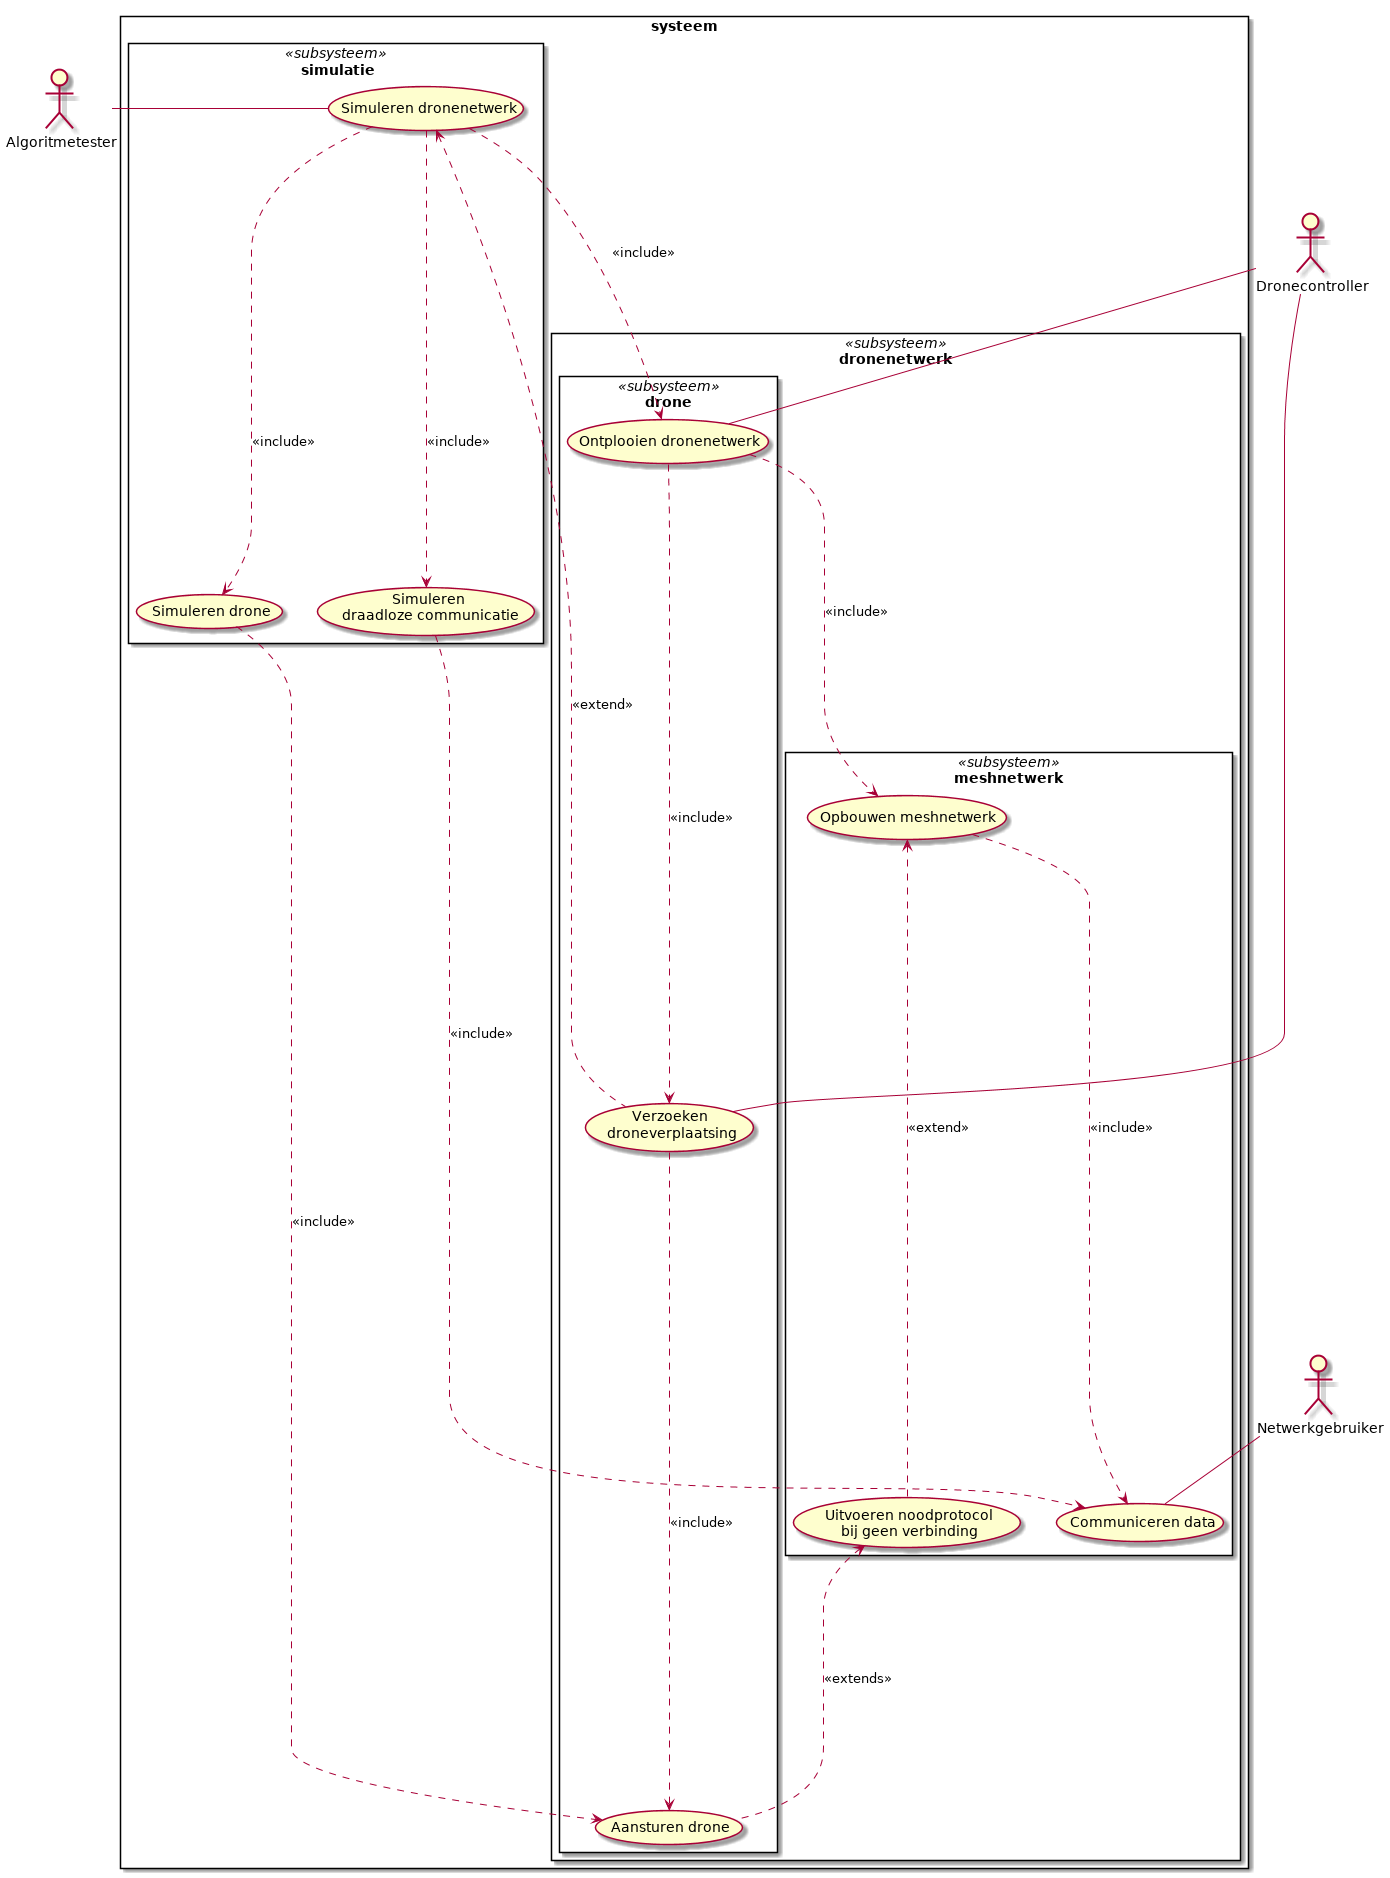
\includegraphics[width=.9\linewidth]{UML/out/usecase/usecasediagram/usecasediagram.png}\end{center}
	\caption{Usecase diagram}
	\label{fig:usecasediagram}
\end{figure}

\begin{table}[H]
	\centering
	\begin{tabular}{|l|l|}
		\hline
		\rowcolor[HTML]{C0C0C0} 
		Usecase & Beschrijving \\ \hline
		\nameref{Usecase:simulatiedronenetwerk} & \begin{tabular}[c]{@{}l@{}}Een actor wil een dronenetwerk simuleren hiervoor moeten\\ drones en draadloze communicatie gesimuleerd worden.\end{tabular} \\ \hline
		\nameref{Usecase:simulatiedrone} & Het systeem gaat een drone simuleren. \\ \hline
		\hyperlink{draadlozecom}{\begin{tabular}[c]{@{}l@{}}Simuleren draadloze \\ communicatie\end{tabular}} & \begin{tabular}[c]{@{}l@{}}Het systeem gaat draadloze communicatie simuleren. \\ Hiermee kan het data communiceren.\end{tabular} \\ \hline
		\nameref{Usecase:communicerendata} & \begin{tabular}[c]{@{}l@{}}Een actor geeft aan dat hij data wil communiceren via het\\ netwerk.\end{tabular} \\ \hline
		\nameref{Usecase:opbouwenmeshnetwerk} & \begin{tabular}[c]{@{}l@{}}Het systeem gaat een mesh netwerk opbouwen tussen \\ aanwezige nodes.\end{tabular} \\ \hline
		\hyperlink{noodprotocol}{\begin{tabular}[c]{@{}l@{}}Uitvoeren noodprotocol \\ bij geen verbinding\end{tabular}} & \begin{tabular}[c]{@{}l@{}}Het systeem gaat wanneer er een bepaalde tijd geen\\ verbinding is met een gateway een noodprotocol uitvoeren\\ om het meshnetwerk te herstellen.\end{tabular} \\ \hline
		\nameref{Usecase:ontplooien} & \begin{tabular}[c]{@{}l@{}}Een actor wil een dronenetwerk ontplooien over een gebied \\ hiervoor worden  drones aangestuurd.\end{tabular} \\ \hline
		\nameref{Usecase:verzoekverplaatsing} & Een actor stuurt een verzoek tot het verplaatsen van een drone. \\ \hline
		\nameref{Usecase:aansturendrone} & \begin{tabular}[c]{@{}l@{}}Het systeem stuurt een drone aan om zich te verplaatsen naar\\ een locatie.\end{tabular} \\ \hline
	\end{tabular}
	\caption{Korte toelichting usecases}
	\label{tab:toelichtingusecase}
\end{table}


\chapter{Domein Model}
\label{domeinmodel}

Aan de hand van een domeinmodel wordt de samenhang van de te ontwikkelen software in kaart gebracht.
In de hier opvolgende \nameref{domeinmodel:beschrijving} wordt per class toelichting gegeven.

\begin{figure}[H]
	\begin{center}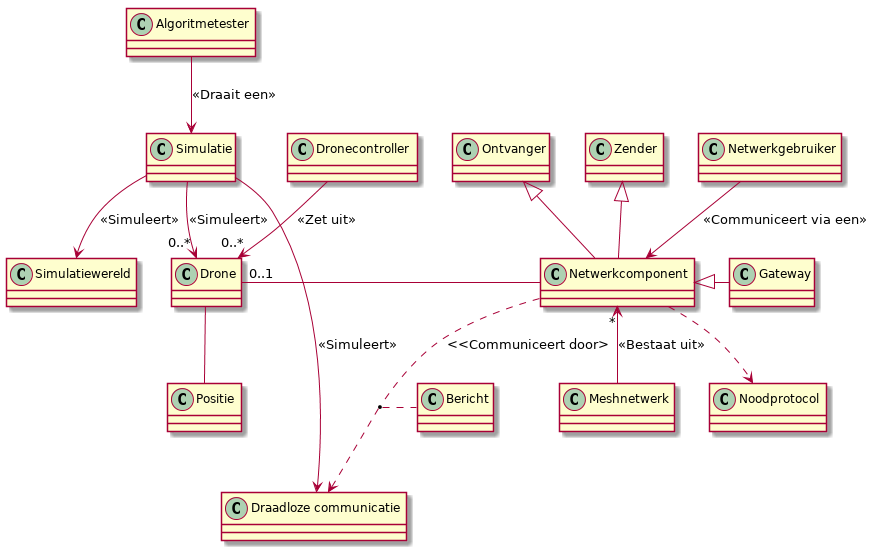
\includegraphics[height=.65\textheight]{UML/out/DomeinModel/DomeinModel/DomeinModel.png}\end{center}
	\caption{Domeinmodel}
	\label{fig:toplogienetwerkuml}
\end{figure}

\section{Beschrijving domeinmodel}
\label{domeinmodel:beschrijving}

% Please add the following required packages to your document preamble:
% \usepackage[table,xcdraw]{xcolor}
% If you use beamer only pass "xcolor=table" option, i.e. \documentclass[xcolor=table]{beamer}
% \usepackage{longtable}
% Note: It may be necessary to compile the document several times to get a multi-page table to line up properly
\begin{longtable}[c]{|l|l|}
	\hline
	\rowcolor[HTML]{C0C0C0} 
	Naam & Beschrijving \\ \hline
	\endfirsthead
	%
	\multicolumn{2}{c}%
	{{\bfseries Table \thetable\ continued from previous page}} \\
	\endhead
	%
	gazebo & Gazebo is de simulatie omgeving voor physics \\ \hline
	Drone & \begin{tabular}[c]{@{}l@{}}Een drone kan zichzelf verplaatsen in een ruimte \\ met een DroneEngine\end{tabular} \\ \hline
	DroneEngine & \begin{tabular}[c]{@{}l@{}}Een drone engine wordt gebruikt door de drone \\ voor verplaatsing\end{tabular} \\ \hline
	RouterDrone & \begin{tabular}[c]{@{}l@{}}Een RouterDrone is een drone voorzien van een \\ ArduinoRouter\end{tabular} \\ \hline
	GatewayDrone & \begin{tabular}[c]{@{}l@{}}Een RouterGateway is een drone voorzien van \\ een ArduinoGateway\end{tabular} \\ \hline
	Arduino & Een arduino is een mircocontrollerbord \\ \hline
	ArduinoRouter & \begin{tabular}[c]{@{}l@{}}Is een arduino voorzien van MeshnetworkRouter \\ software\end{tabular} \\ \hline
	ArduinoGateway & \begin{tabular}[c]{@{}l@{}}Is een arduino voorzien van MeshnetworkGateway \\ software\end{tabular} \\ \hline
	MeshnetworkComponent & Is een onderdeel binnen een meshnetwerk \\ \hline
	MeshnetworkRouter & \begin{tabular}[c]{@{}l@{}}Is een meshcomponent in staat berichten binnen het\\ netwerk door te sturen\end{tabular} \\ \hline
	MeshnetworkGateway & \begin{tabular}[c]{@{}l@{}}Is een meshcomponent met een verbinding extern \\ van het netwerk\end{tabular} \\ \hline
	InternetConnection & Is een  verbinding naar het wereldwijde web \\ \hline
	DroneManager & Een manager voor het aansturen van drones \\ \hline
	ros & \begin{tabular}[c]{@{}l@{}}Middleware voor het aansturen van fysieke of\\  gesimuleerde drones\end{tabular} \\ \hline
	Message & Een bericht gebruikt voor communicatie \\ \hline
	WirelessCommunication & Communicatie type die door de lucht verloopt \\ \hline
	NRF24 & Een radio transceiver bruikbaar voor communicatie \\ \hline
	\caption{Toelichting domeinmodel}
	\label{tab:domeinmodel}\\
\end{longtable}


\chapter{Use-case omschrijvingen}
\label{Usecase}

\section[Simuleren dronenetwerk]{Usecase: Simuleren dronenetwerk}
\label{Usecase:simulatiedronenetwerk}
\subsection{Fully-dressed usecase description}

\begin{table}[H]
	\centering
	\begin{tabular}{|l|}
		\hline
		Usecase: Simuleren dronenetwerk 				                                                                             \\ \hline
		Doel: De actor wil een dronenetwerk simuleren om algritmes te testen zonder fysieke drones                                    \\ \hline
		\begin{tabular}[c]{@{}l@{}}Beschrijving van de usecase:  De usecase start een simulatie op waarin een instelbaar aantal\\
								 drones gesimuleerd worden welke onderling kunnen communiceren via een gesimuleerde\\
								 draadloze communicatieweg. Hiermee creëren zij een meshnetwerk. \end{tabular} \\ \hline
		Primary actor:  \nameref{inleiding:gebruikers:algoritmetester}                                                               \\ \hline
		Preconditions: Er is aangegeven hoeveel routers en gateway gesimuleerd moeten worden.                                         \\ \hline
		Postconditions: De simulatie van de drones en de communicatie is opgestart                                                     \\ \hline
	\end{tabular}
\end{table}

\subsection{Basic Flow}
\begin{table}[H]
	\centering
	\begin{tabular}{|l|l|}
		\hline
		\rowcolor[HTML]{C0C0C0} 
		Actor actie  & System responsibility   \\ \hline
		1. Start de applicatie.& 2. Leest het configuratie bestand uit. \\ \hline
		& 3. Start de wereld simulatie.                     \\ \hline
		& 4. Start de communicatie simulatie.                     \\ \hline
		& 5. Laadt het opgegeven aantal gatewaydrones de simulatie in.                         \\ \hline
		& 6. Laadt opgegeven aantal routerdrones de simulatie in.                         \\ \hline
		& 7. Start de dronemanager.                 \\ \hline
	\end{tabular}
\end{table}


\label{Usecase:simulatiedronenetwerk:fully-dressed}
\subsection{System Sequence Diagram}
\label{Usecase:simulatiedronenetwerk:systemsequence}
\begin{figure}[H]
	\begin{center}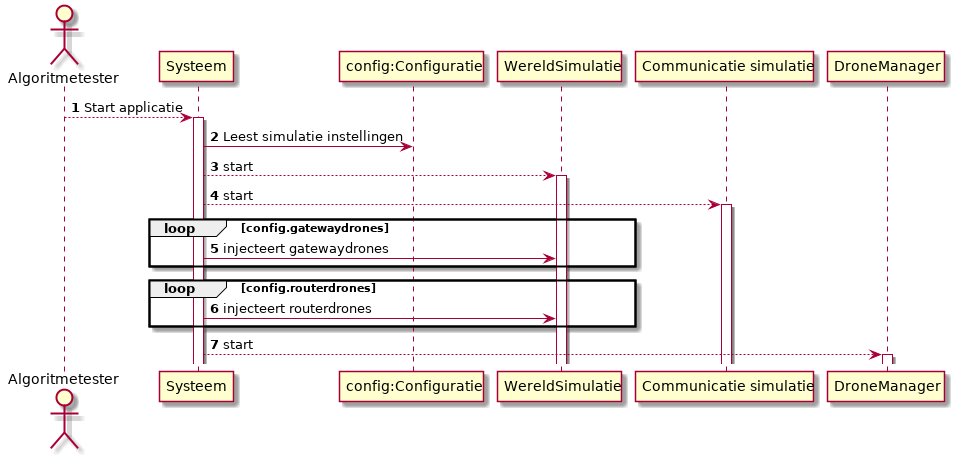
\includegraphics[height=.3\textheight]{UML/out/usecase/sequence/SimulerenDronenetwerk/SimulerenDronenetwerk.png}\end{center}
	\caption{System sequence diagram opstarten simulatie}
	\label{fig:simulatiedronenetwerk:systemsequence}
\end{figure}


\section[Simuleren drone]{Usecase: Simuleren drone}
\label{Usecase:simulatiedrone}
\subsection{Fully-dressed usecase description}

\begin{table}[H]
	\centering
	\begin{tabular}{|l|}
		\hline
		Usecase: Simuleren drone.                                                                            \\ \hline
		Doel: Het creëren van een virtuele representatie van een drone.                                                                \\ \hline
		\begin{tabular}[c]{@{}l@{}}Beschrijving van de usecase: In de simulatie wil een actor een drone simuleren.\\
									Door het uitvoeren van deze usecase wordt er een drone in de simulatie geladen\\
									welke de rol van gateway of router kan hebben. \\ \end{tabular} \\ \hline
		Primary actor:  \nameref{Usecase:simulatiedronenetwerk}                                                                                \\ \hline
		Preconditions: Er is een simulatiewereld aanwezig.                                                                         \\ \hline
		Postconditions: Een drone is ingeladen in de simulatiewereld.                                                     \\ \hline
	\end{tabular}
\end{table}

\subsection{Basic Flow }

\begin{table}[H]
	\centering
	\begin{tabular}{|l|l|}
		\hline
		\rowcolor[HTML]{C0C0C0} 
		Actor action  & System responsibility   \\ \hline
		1. Leest configuratie uit.  & 						  \\ \hline
		2. Verzoekt het injecteren van een gatewaydrone.	& 3. Leest de drone parameters uit.                          \\ \hline
											& 4. Koppelt een motor aan de gesimuleerde drone.                         \\ \hline
											& 	\begin{tabular}[c]{@{}l@{}}5. Koppelt een gatewaycomponent aan de\\ gesimuleerde drone. \\ \end{tabular} \\ \hline
											& 6. Injecteert de drone de gesimuleerde wereld in.                         \\ \hline
	\end{tabular}
\end{table}

\subsection{Alternative Flows}

\begin{table}[H]
	\centering
	\begin{tabular}{|l|l|}
		\hline
		\rowcolor[HTML]{C0C0C0} 
		Actor action  & System responsibility   \\ \hline
		2. Verzoekt het injecteren van een routerdrone.	& 3. Leest de drone parameters uit.                          \\ \hline
& 	\begin{tabular}[c]{@{}l@{}}5. Koppelt een router component aan de\\ gesimuleerde drone. \\ \end{tabular} \\ \hline 
	\end{tabular}
\end{table}

\label{Usecase:simulatiedrone:fully-dressed}
\subsection{System Sequence Diagram}
\label{Usecase:simulatiedrone:systemsequence}

\begin{figure}[H]
	\begin{center}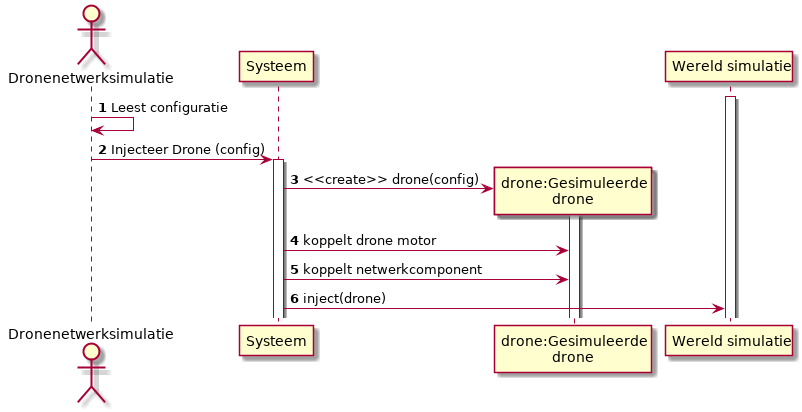
\includegraphics[height=.3\textheight]{UML/out/usecase/sequence/SimulerenDrone/SimulerenDrone.png}\end{center}
	\caption{System sequence diagram opstarten drone simulatie}
	\label{fig:simulatiedrone:systemsequence}
\end{figure}

\hypertarget{draadlozecom}{
\section[Simuleren draadloze communicatie]{Usecase: Simuleren draadloze communicatie}}
\label{Usecase:simmulatiecommuicatie}
\subsection{Fully-dressed usecase description}

\begin{table}[H]
	\centering
	\begin{tabular}{|l|}
		\hline
		Use Case: Simuleren draadloze communicatie.                                                                            \\ \hline
		Doel: Het nabootsen van draadloze communicatie in een simulator.                               \\ \hline
		\begin{tabular}[c]{@{}l@{}}Beschrijving van de usecase: In de simulatie wil een actor gebruik maken van\\
								draadloze communicatie. Om dit realistisch na te bootsen loopt elk bericht langs\\
								de draadloos simulator die bepaalt wat er met het bericht gebeurd.\\ \end{tabular} \\ \hline
		Primary actor:  \nameref{Usecase:simulatiedronenetwerk}.                                                                                \\ \hline
		Preconditions:                                                                          \\ \hline
		\begin{tabular}[c]{@{}l@{}}Postconditions: Er is een simulator aanwezig die \nameref{Usecase:communicerendata} mogelijk\\maakt voor gesimuleerde \nameref{inleiding:werkomgeving:nrf24}'s.  \\ \end{tabular}   \\ \hline
	\end{tabular}
\end{table}

\subsection{Basic Flow}

\begin{table}[H]
	\centering
	\begin{tabular}{|l|l|}
		\hline
		\rowcolor[HTML]{C0C0C0} 
		Actor action  & System responsibility   \\ \hline
		\begin{tabular}[c]{@{}l@{}}1. Start applicatie met\\ maximale afstand parameter.{}\end{tabular}&\begin{tabular}[c]{@{}l@{}}2. Stelt de meegegeven waarde in voor de\\ maximale communicatie afstand. {}\end{tabular}\\ \hline
		& 3. Start draadloze simulator.                  \\ \hline
		
	\end{tabular}
\end{table}

\subsection{Alternative Flows}

\begin{table}[H]
	\centering
	\begin{tabular}{|l|l|}
		\hline
		\rowcolor[HTML]{C0C0C0} 
		Actor action  & System responsibility   \\ \hline
		\begin{tabular}[c]{@{}l@{}}1. Start applicatie zonder\\ parameters.{}\end{tabular}&\begin{tabular}[c]{@{}l@{}}2. Stelt de standaard waarde in voor de\\ maximale communicatie afstand. {}\end{tabular}\\ \hline
	\end{tabular}
\end{table}

\label{Usecase:simmulatiecommuicatie:fully-dressed}
\subsection{System Sequence Diagram }
\label{Usecase:simmulatiecommuicatie:systemsequence}

\begin{figure}[H]
	\begin{center}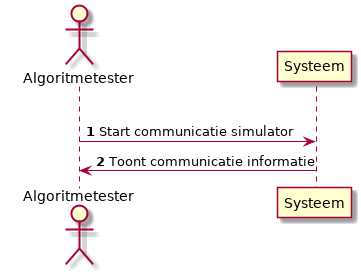
\includegraphics[height=.3\textheight]{UML/out/usecase/sequence/Simulerendraadlozecommunicatie/Simulerendraadlozecommunicatie.png}\end{center}
	\caption{System sequence diagram opstarten draadloze communicatie simulatie}
	\label{fig:simmulatiecommuicatie:systemsequence}
\end{figure}

\section[Communiceren data]{Use case: Communiceren data}
\label{Usecase:communicerendata}
\subsection{Fully-dressed usecase description}
\label{Usecase:communicerendata:fully-dressed}
\begin{table}[H]
	\centering
	\begin{tabular}{|l|}
		\hline
		Use Case: Communiceren data.					                                                                              \\ \hline
		Purpose: Deze usecase wordt gebruiken om data uit te wisselen tussen componenten                                             \\ \hline
		\begin{tabular}[c]{@{}l@{}}Beschrijving van de usecase: In het netwerk zullen componenten met elkaar willen \\communiceren. Deze usecase zal de data proberen te versturen. \\ \end{tabular} \\ \hline
		Primary actor:  \nameref{inleiding:gebruikers:netwerkgebruiker}, \nameref{Usecase:simmulatiecommuicatie}, \nameref{Usecase:opbouwenmeshnetwerk}                       \\ \hline
		 \begin{tabular}[c]{@{}l@{}}Preconditions: Communicatiemiddel van de zender is opgestart, de te versturen data is bekend,\\ en het adres van de ontvanger is bekend.{}\end{tabular}\\ \hline
		Postconditions: Er is data verstuurd van een component naar een andere component.                                           \\ \hline
	\end{tabular}
\end{table}

\subsection{Basic Flow }

\begin{table}[H]
	\centering
	\begin{tabular}{|l|l|}
		\hline
		\rowcolor[HTML]{C0C0C0} 
		Actor action  & System responsibility   \\ \hline
		1. Geeft bericht om te verzenden & 2. Zet bericht om in overdraagbare data  \\ \hline
		& 3. Opent verbinding met ontvanger                         \\ \hline
		& 4. Verstuurd bericht naar ontvanger                        \\ \hline
5. Krijgt notificatie van slagen & 6. Ontvangend syteem zet data terug naar bericht \\ \hline
		 & 7. Ontvanger ontvangt bericht                         \\ \hline
	\end{tabular}
\end{table}

\subsection{Alternative Flows}

\begin{table}[H]
	\centering
	\begin{tabular}{|l|l|}
		\hline
		\rowcolor[HTML]{C0C0C0} 
		Actor action  & System responsibility   \\ \hline
		& 3. Kan geen verbinding openen met ontvanger                        \\ \hline
	4. Krijgt notificatie van het niet slagen	&                         \\ \hline
	\end{tabular}
\end{table}



\subsection{System Sequence Diagram }
\label{Usecase:communicerendata:systemsequence}

\begin{figure}[H]
	\begin{center}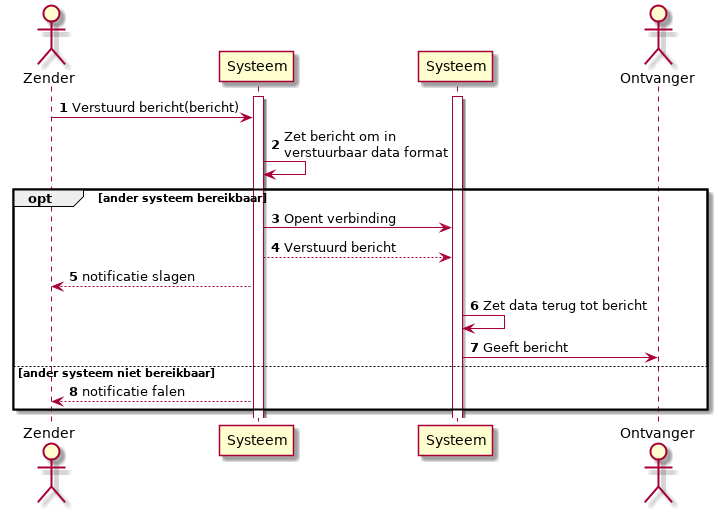
\includegraphics[height=.4\textheight]{UML/out/usecase/sequence/VersturenBericht/VersturenBericht.png}\end{center}
	\caption{System sequence diagram opstarten draadloze communicatie simulatie}
	\label{fig:communicerendata:systemsequence}
\end{figure}

\section[Opbouwen meshnetwerk]{Usecase : Opbouwen meshnetwerk}
\label{Usecase:opbouwenmeshnetwerk}
\subsection{Fully-dressed usecase description}

\begin{table}[H]
	\centering
	\begin{tabular}{|l|}
		\hline
		Usecase: Opbouwen meshnetwerk				                                                                              \\ \hline
		\begin{tabular}[c]{@{}l@{}} Doel: Het uitvoeren van de usecase zal een netwerk opzetten van onderling\\ verbonden meshnetwerkcomponenten.{}\end{tabular}  \\ \hline
		\begin{tabular}[c]{@{}l@{}}Beschrijving van de usecase:  Na het uitvoeren van de usecase moeten alle\\ meshnetwerkcomponenten een verbinding hebben met de netwerkcomponenten die\\ binnen hun bereik zijn. De componenten staan klaar om berichten door te sturen \\naar elkaar of naar een gateway voor externe adressen.{}\end{tabular} \\ \hline
		Primary actor:  \nameref{Usecase:ontplooien}                                                                                \\ \hline
		\begin{tabular}[c]{@{}l@{}} Preconditions: Componenten zijn binnen bereik van elkaar, er is minstens één \\gateway aanwezig.{}\end{tabular}		                      \\ \hline
		Postconditions: Er is een onderling verbonden netwerk opgebouwd.                                                                       \\ \hline
	\end{tabular}
\end{table}

\subsection{Basic Flow }


\begin{table}[H]
	\centering
	\begin{tabular}{|l|l|}
		\hline
		\rowcolor[HTML]{C0C0C0} 
		Actor action  & System responsibility   \\ \hline
		1. Start applicatie. & 2. Start communicatie methode. \\ \hline
		& 3. Componenten maken verbinding met elkaar.  \\ \hline
		& 4. Componenten berekenen verbindingspaden        \\ \hline
		& 5. Maak contact met extern adres. \\ \hline
	\end{tabular}
\end{table}

\subsection{Alternative Flows}


\begin{table}[H]
	\centering
	\begin{tabular}{|l|l|}
		\hline
		\rowcolor[HTML]{C0C0C0} 
		Actor action  & System responsibility   \\ \hline
		& 3. Componenten maken geen directe of indirecte verbinding met een gateway.\\ \hline
		& 4. Componenten starten \nameref{Usecase:noodprotocol}.      \\ \hline
	\end{tabular}
\end{table}

\label{Usecase:opbouwenmeshnetwerk:fully-dressed}
\subsection{System Sequence Diagram }
\label{Usecase:opbouwenmeshnetwerk:systemsequence}

\begin{figure}[H]
	\begin{center}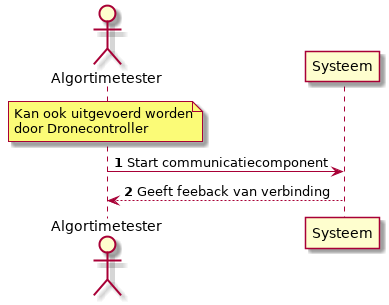
\includegraphics[height=.3\textheight]{UML/out/usecase/sequence/meshnetwerk/meshnetwerk.png}\end{center}
	\caption{System sequence diagram opzetten meshnetwerk.}
	\label{fig:opbouwenmeshnetwerk:systemsequence}
\end{figure}


\hypertarget{noodprotocol}{\section[Uitvoeren noodprotocol bij geen verbinding]{Use case: Uitvoeren noodprotocol bij geen verbinding}}
\label{Usecase:noodprotocol}
\subsection{Fully-dressed usecase description}
\label{Usecase:noodprotocol:fully-dressed}

\begin{table}[H]
	\centering
	\begin{tabular}{|l|}
		\hline
		Use Case: Uitvoeren noodprotocol bij geen verbinding                                                                              \\ \hline
		\begin{tabular}[c]{@{}l@{}}Doel: Door het uitvoeren van een noodprotocol zijn één of meerdere drones in staat\\de verbinding te herstellen met een gateway. Hiervoor kan het gebruik maken van\\ \nameref{Usecase:aansturendrone}.{}\end{tabular}\\ \hline
		\begin{tabular}[c]{@{}l@{}}Beschrijving van de usecase: Deze usecase is de uiterste stap die een meshcomponent.{}\end{tabular} \\ \hline
		Primary actor:  \nameref{Usecase:opbouwenmeshnetwerk}                                                                                \\ \hline
		Preconditions: 	Elke drone heeft ooit direct of indirect verbinding gehad met een gateway.		                                                                          \\ \hline
		Postconditions: Drone(s) is/zijn herplaatst naar een positie in verbinding met een gateway. \\ \hline
	\end{tabular}
\end{table}

\subsection{Basic Flow }


\begin{table}[H]
	\centering
	\begin{tabular}{|l|l|}
		\hline
		\rowcolor[HTML]{C0C0C0} 
		Actor action  & System responsibility   \\ \hline
		1. Start noodprotocol. &  2. Kijkt of node alleen is of samen.\\ \hline
						   	&  3. Drones bepalen verplaatsing.     \\ \hline
						    &  4. Drones herpositioneren zich.	    \\ \hline
							&  5. Alle drones hebben direct of indirect verbinding met een gateway.\\ \hline
	\end{tabular}
\end{table}

\subsection{Alternative Flows}


\begin{table}[H]
	\centering
	\begin{tabular}{|l|l|}
		\hline
		\rowcolor[HTML]{C0C0C0} 
		Actor action  & System responsibility   \\ \hline
	    &  3. Enkele drone bepaalt verplaatsing.     \\ \hline
        &  4. Enkele drones herpositioneert zich.	    \\ \hline
	\end{tabular}
\end{table}

\begin{table}[H]
	\centering
	\begin{tabular}{|l|l|}
		\hline
		\rowcolor[HTML]{C0C0C0} 
		Actor action  & System responsibility   \\ \hline
		&  5. Drone(s) heeft/hebben nog geen verbinding met gateway.     \\ \hline
		&  6. Drone(s) verplaatst/verplaatsen zich terug naar positie van gateway.	    \\ \hline
	\end{tabular}
\end{table}

\subsection{System Sequence Diagram }
\label{Usecase:noodprotocol:systemsequence}

\begin{figure}[H]
	\begin{center}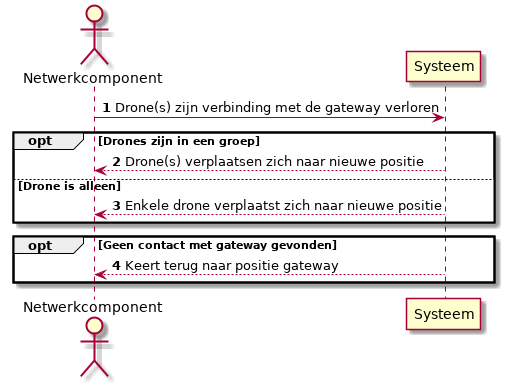
\includegraphics[height=.4\textheight]{UML/out/usecase/sequence/noodprotocol/noodprotocol.png}\end{center}
	\caption{System sequence diagram noodprotocol.}
	\label{fig:noodprotocol:systemsequence}
\end{figure}


\section[Ontplooien dronenetwerk]{Usecase: Ontplooien dronenetwerk}
\label{Usecase:ontplooien}
\subsection{Fully-dressed usecase description}
\label{Usecase:ontplooien:fully-dressed}

\begin{table}[H]
	\centering
	\begin{tabular}{|l|}
		\hline
		Use Case:Ontplooien dronenetwerk                                                                             \\ \hline
		\begin{tabular}[c]{@{}l@{}}Doel: Het doel van deze usecase is het ontplooien van een dronenetwerk, met\\een casus zal worden aangegeven waar naartoe te verplaatsen, ze moeten\\ zelfstandig een netwerk opzetten.{}\end{tabular}   \\ \hline
		\begin{tabular}[c]{@{}l@{}}Beschrijving van de usecase: Deze usecase zal alle drones aansturen om naar\\ een vooraf bepaalde posities te vliegen. De drones zullen een meshnetwerk\\ opbouwen waarover gecommuniceerd kan worden. \\ \end{tabular} \\ \hline
		Primary actor:  \nameref{inleiding:gebruikers:dronecontroller}, \nameref{Usecase:simulatiedronenetwerk}  \\ \hline
		\begin{tabular}[c]{@{}l@{}}Preconditions: Drones zijn voorzien van meshcomponenten en kunnen zich\\verplaatsen. Er zijn genoeg drones aanwezig voor de casus. {}\end{tabular} \\ \hline
		\begin{tabular}[c]{@{}l@{}}Postconditions: Drones zijn verplaatst naar ingestelde positie en hebben\\een onderling netwerk opgebouwd.{}\end{tabular} \\ \hline
	\end{tabular}
\end{table}

\subsection{Basic Flow }


\begin{table}[H]
	\centering
	\begin{tabular}{|l|l|}
		\hline
		\rowcolor[HTML]{C0C0C0} 
		Actor action  & System responsibility   \\ \hline
		1. Start alle netwerkdrones op. 		& \\ \hline
		2. Geeft posities door voor de drones.  & 3. Stuurt elke individuele drone aan naar positie.    \\ \hline
												& 4. Meshcomponenten bouwen netwerk op.                 \\ \hline
	\end{tabular}
\end{table}

\subsection{Alternative Flows}


\begin{table}[H]
	\centering
	\begin{tabular}{|l|l|}
		\hline
		\rowcolor[HTML]{C0C0C0} 
		Actor action  & System responsibility   \\ \hline
		& 3. Er zijn niet genoeg drones voor de casus aanwezig of binnen bereik    \\ \hline
		& 4. De drones die wel bereikbaar zijn verplaatsen zich.      	    \\ \hline
	\end{tabular}
\end{table}

\subsection{System Sequence Diagram }
\label{Usecase:ontplooien:systemsequence}


\begin{figure}[H]
	\begin{center}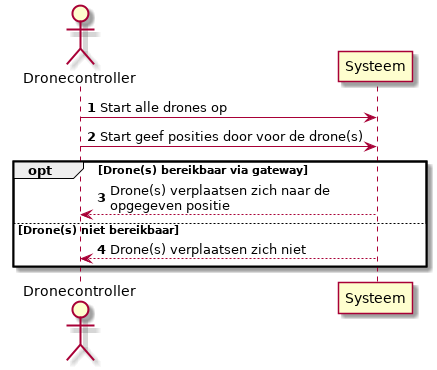
\includegraphics[height=.4\textheight]{UML/out/usecase/sequence/ontplooien/ontplooien.png}\end{center}
	\caption{System sequence diagram noodprotocol.}
	\label{fig:ontplooien:systemsequence}
\end{figure}


\section[Verzoeken droneverplaatsing]{Usecase: Verzoeken droneverplaatsing}
\label{Usecase:verzoekverplaatsing}
\subsection{Fully-dressed usecase description}
\label{Usecase:verzoekverplaatsing:fully-dressed}
\begin{table}[H]
	\centering
	\begin{tabular}{|l|}
		\hline
		Usecase: Verzoeken droneverplaatsing                                                                              \\ \hline
		Doel: Deze usecase dient voor het verzoeken tot een verplaatsing van een drone.                                    \\ \hline
		\begin{tabular}[c]{@{}l@{}}Beschrijving usecase: Door deze usecase te gebruiken kan een individuele\\drone verzocht worden zich te verplaatsen.  {}\end{tabular} \\ \hline
		Primary actor:  \nameref{inleiding:gebruikers:dronecontroller}, \nameref{Usecase:simulatiedronenetwerk}, \nameref{Usecase:ontplooien}. \\ \hline
		Preconditions: Communicatieweg beschikbaar tot aan drone.\\ \hline
		Postconditions: Drone gaat zich verplaatsen naar verzoeklocatie.            \\ \hline
	\end{tabular}
\end{table}

\subsection{Basic Flow }


\begin{table}[H]
	\centering
	\begin{tabular}{|l|l|}
		\hline
		\rowcolor[HTML]{C0C0C0} 
		Actor action  & System responsibility   \\ \hline
		1. Verstuurt verzoek voor verplaatsing.  & 2. Verstuurt verzoek naar drone. \\ \hline
												 & 3. Stuurt drone aan.  	   \\ \hline
	\end{tabular}
\end{table}

\subsection{Alternative Flows}


\begin{table}[H]
	\centering
	\begin{tabular}{|l|l|}
		\hline
		\rowcolor[HTML]{C0C0C0} 
		Actor action  & System responsibility   \\ \hline
	    & 2. Drone is niet bereikbaar. \\ \hline
	\end{tabular}
\end{table}


\subsection{System Sequence Diagram }
\label{Usecase:verzoekverplaatsing:systemsequence}

\begin{figure}[H]
	\begin{center}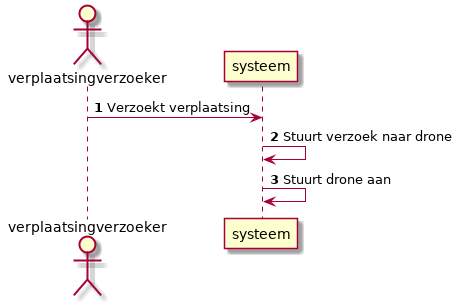
\includegraphics[height=.3\textheight]{UML/out/usecase/sequence/verzoekendroneverplaatsing/verzoekendroneverplaatsing.png}\end{center}
	\caption{System sequence verzoeken verplaatsing.}
	\label{fig:verzoekverplaatsing:systemsequence}
\end{figure}


\section[Aansturen drone]{Usecase: Aansturen drone}
\label{Usecase:aansturendrone}
\subsection{Fully-dressed usecase description}
\label{Usecase:aansturendrone:fully-dressed}
\begin{table}[H]
	\centering
	\begin{tabular}{|l|}
		\hline
		Use Case: Aansturen drone                                                                              \\ \hline
		Purpose: Het aansturen van een drone wordt gebruikt om een drone te verplaatsen.                                                                               \\ \hline
		\begin{tabular}[c]{@{}l@{}}Beschrijving van de usecase: Elke drone kan aangestuurd worden om zicht te verplaatsen.\\Die wordt altijd uitgevoerd vanaf het aangesloten netwerkcomponent. Daarom moet er\\vanuit een extern punt altijd een verzoek gestuurd worden voor een verplaatsing of vanaf de\\aangesloten module zelf komen. {}\end{tabular} \\ \hline
		Primary actor: \nameref{Usecase:verzoekverplaatsing}, \nameref{Usecase:noodprotocol}.                                        \\ \hline
		Preconditions: Drone is in staat zich te verplaatsen                                                                         \\ \hline
		Postconditions: Drone heeft zich verplaatst naar de verzochte positie.                                                                   \\ \hline
	\end{tabular}
\end{table}

\subsection{Basic Flow }


\begin{table}[H]
	\centering
	\begin{tabular}{|l|l|}
		\hline
		\rowcolor[HTML]{C0C0C0} 
		Actor action  & System responsibility   \\ \hline
		1. Stuurt doellocatie & 2. Berekend pad naar locatie \\ \hline
 							  & 3. Start motor \\ \hline
 							  & 4. Verplaatst zich naar locatie \\ \hline
 							  & 5. Stopt motor  \\ \hline
	\end{tabular}
\end{table}

\subsection{Alternative Flows}


\begin{table}[H]
	\centering
	\begin{tabular}{|l|l|}
		\hline
		\rowcolor[HTML]{C0C0C0} 
		Actor action  & System responsibility   \\ \hline
				      & 3. Geen pas mogelijk naar locatie \\ \hline
					  & 4. Blijft op huidige locatie                        \\ \hline
	\end{tabular}
\end{table}


\subsection{System Sequence Diagram }
\label{Usecase:aansturendrone:systemsequence}


\begin{figure}[H]
	\begin{center}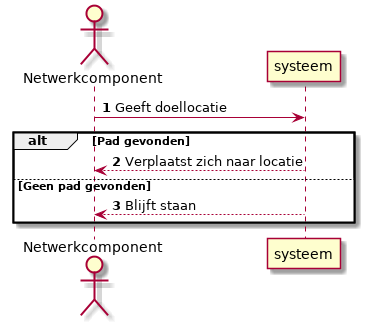
\includegraphics[height=.3\textheight]{UML/out/usecase/sequence/aansturendrone/aansturendrone.png}\end{center}
	\caption{System sequence aansturen drone.}
	\label{fig:aansturendrone:systemsequence}
\end{figure}


\chapter{functionele requirements }
Voor dit project zijn er requirements opgesteld. Deze requirements zijn opgesteld a.d.h.v. de MoSCoW methode, hiervoor is gekozen om de requirements
te prioriteren. De Must requirements moeten voor het einde van het project gerealiseerd worden. De overige requirements hebben een lagere prioriteit en
hieraan wordt pas gewerkt als alle Must requirements afgehandeld zijn. Onder de tabel is per requirement een toelichting te vinden.
\begin{longtable}{|l|l|l|l|}
	\hline
	\rowcolor[HTML]{C0C0C0} 
	Naam & Beschrijving & MoSCoW\\ \hline
	%\endfirsthead
	%
	\endhead
	\hyperlink{SIMULATIE1}{SIMULATIE1}			&\begin{tabular}[c]{@{}l@{}}Simulatie representeert een wereld.	\end{tabular} 							 &M \\ \hline
	\hyperlink{SIMULATIE2}{SIMULATIE2}			&\begin{tabular}[c]{@{}l@{}}Simulatie simuleert en visualiseert een abstracte drone.\end{tabular}        &M \\ \hline
	\hyperlink{SIMULATIE3}{SIMULATIE3}			&\begin{tabular}[c]{@{}l@{}}Simulatie simuleert de beweging van een drone.\end{tabular}       			 &M \\ \hline
	\hyperlink{SIMULATIE4}{SIMULATIE4}			&\begin{tabular}[c]{@{}l@{}}Simulatie simuleert tot 100 drones tegelijk.\end{tabular}        			 &S \\ \hline	
	\hyperlink{SIMULATIE5}{SIMULATIE5}			&\begin{tabular}[c]{@{}l@{}}Simulatie simuleert draadloze communicatie.\end{tabular}        			 &M \\ \hline	
	\hyperlink{SIMULATIE6}{SIMULATIE6}			&\begin{tabular}[c]{@{}l@{}}Simulatie simuleert een Arduino. \end{tabular}        						 &S \\ \hline	
	\hyperlink{SIMULATIE7}{SIMULATIE7}			&\begin{tabular}[c]{@{}l@{}}Simulatie kan met een configuratiebestand gestart worden. \end{tabular}     &S \\ \hline	
	\hyperlink{DRONE1}{DRONE1}		&\begin{tabular}[c]{@{}l@{}}Drone kan zich verplaatsen naar een positie. \end{tabular}        			 &M \\ \hline	
	\hyperlink{DRONE2}{DRONE2}		&\begin{tabular}[c]{@{}l@{}}Drone kan een route naar positie berekenen.  \end{tabular}        			 &S \\ \hline	
	\hyperlink{DRONE3}{DRONE3}		&\begin{tabular}[c]{@{}l@{}}Drone kan een locatie aanbieden.  \end{tabular}        						 &M \\ \hline	
	\hyperlink{DRONE4}{DRONE4}		&\begin{tabular}[c]{@{}l@{}}Drone is voorzien van een netwerkcomponent.  \end{tabular}       &M \\ \hline	
	\hyperlink{NETWERK1}{NETWERK1}	&\begin{tabular}[c]{@{}l@{}}Netwerk kan zelfstandig een meshnetwerk opbouwen. \end{tabular}    			 &M \\ \hline	
	\hyperlink{NETWERK2}{NETWERK2}	&\begin{tabular}[c]{@{}l@{}}Netwerk heeft altijd minstens 1 gateway. 	\end{tabular}			 &M \\ \hline	
	\hyperlink{NETWERK3}{NETWERK3}	&\begin{tabular}[c]{@{}l@{}}Netwerk kan drones aansturen.						 \end{tabular}			 &M \\ \hline	
	\hyperlink{NETWERK4}{NETWERK4}	&\begin{tabular}[c]{@{}l@{}}Netwerk biedt een externe interface voor aansturing aan. \end{tabular}		 &S \\ \hline	
	\hyperlink{NETWERK5}{NETWERK5}	&\begin{tabular}[c]{@{}l@{}}Netwerk kan onderling data communiceren.	 \end{tabular}					 &M \\ \hline	
	\hyperlink{NETWERK6}{NETWERK6}	&\begin{tabular}[c]{@{}l@{}}Netwerk kan zichzelf herstellen. \end{tabular}			 					 &M \\ \hline	
	\hyperlink{NETWERK7}{NETWERK7}	&\begin{tabular}[c]{@{}l@{}}Meerdere gateways kunnen tegelijk aanwezig zijn in het netwerk. \end{tabular}			 					 &C \\ \hline	
	\hyperlink{ALGORITME1}{ALGORITME1}		&\begin{tabular}[c]{@{}l@{}}Algoritmetester kan drones verdelen. \end{tabular}		 					 &M \\ \hline	
	\hyperlink{ALGORITME2}{ALGORITME2}		&\begin{tabular}[c]{@{}l@{}}Algoritmetester kan een casus met een verdeling starten. \end{tabular}		 					 &C \\ \hline	
	\caption{Functionele requirements}
	\label{tab:criteria}
\end{longtable}

\section{Toelichting functionele requirements}

\subsection{Simulatie}
Onderstaand worden alle functionele requirements van de simulatie toegelicht
\paragraph{SIMULATIE1: Simulatie representeert een wereld}
\hypertarget{SIMULATIE1}{}

De simulatiecomponent moet een echte wereld nabootsen, er hoeven nog geen objecten in aanwezig te zijn.

\paragraph{SIMULATIE2: Simulatie simuleert en visualiseert een abstracte drone.}
\hypertarget{SIMULATIE2}{}

De simulatie moet een abstracte versie van een drone representeren hierbij maakt de vorm niet uit zolang er maar een verschil te zien is tussen het type drone.

\paragraph{SIMULATIE3: Simulatie simuleert de beweging van een drone.}
\hypertarget{SIMULATIE3}{}

De drone moet bewegen in de simulatie het is belangrijk dat deze beweging visueel zichtbaar is voor analyse van het verplaatsingsgedrag.

\paragraph{SIMULATIE4: Simulatie simuleert tot 100 drones tegelijk.}
\hypertarget{SIMULATIE4}{}

Om met meerdere drones te kunnen testen moet de simulatie tot aan honderd drones tegelijk kunnen simuleren dit hoeft niet visueel te gebeuren om de grafische kaart te ontlasten.

\paragraph{SIMULATIE5: Simulatie simuleert draadloze communicatie.}
\hypertarget{SIMULATIE5}{}

Omdat het draait om een simulatie van een meshnetwerk moet er een component aanwezig zijn die zorgt dat de draadloze communicatie volgens de juiste regels verloopt.

\paragraph{SIMULATIE6: Simulatie simuleert een Arduino.}
\hypertarget{SIMULATIE6}{}

In het project wordt gebruik gemaakt van het Arduino microcontroller bord deze moet virtueel gerepresenteerd worden door de simulatie. 

\paragraph{SIMULATIE7: Simulatie kan met een configuratiebestand gestart worden.}
\hypertarget{SIMULATIE7}{}

Om het starten van simulaties gemakkelijk te maken voor de algoritmetester moet het mogelijk zijn simulaties via een configuratie op te starten.

\subsection{Drone}
Onderstaand worden alle functionele requirements van de drone toegelicht.
\paragraph{DRONE1: Drone kan zich verplaatsen naar een positie}
\hypertarget{DRONE1}{}

Het netwerk rekent op de mogelijkheid van een drone om zich te kunnen verplaatsen om zo het herstellend vermogen te vergroten.

\paragraph{DRONE2: Drone kan een route naar positie berekenen}
\hypertarget{DRONE2}{}

Een drone moet op bais van een ontvangen doel zich kunnen verplaatsen naar een positie. Om deze verplaatsingen uit te kunnen voeren maakt hij gebruik van een zelf berekende route.

\paragraph{DRONE3: Drone kan een locatie aanbieden}
\hypertarget{DRONE3}{}

Een netwerkmodule is zelf niet voorzien van een component voor het ophalen van een locatie daarvoor maakt hij gebruik van de drone. Daarom moet een drone in staat zijn om zijn locatie door te geven.

\paragraph{DRONE4: Drone is voorzien van een meshnetwerkcomponent}
\hypertarget{DRONE4}{}

Een drone moet worden voorzien van een meshnetwerkcomponent om zo alle drones wanneer mogelijk met elkaar te kunnen laten communiceren.

\subsection{Netwerk}
Onderstaand worden alle functionele requirements van het netwerk toegelicht.

\paragraph{NETWERK1: Netwerk kan zelfstandig een meshnetwerk opbouwen}
\hypertarget{NETWERK1}{}

De opzetter van het netwerk wil zich niet bezig hoeven houden met het onderling verbinden van de drones. Zij moeten zelf een netwerk opzetten zonder tussenkomst van menselijke actoren.

\paragraph{NETWERK2: Netwerk biedt altijd minstens 1 gateway aan}
\hypertarget{NETWERK2}{}

Om het netwerk toegang te kunnen geven tot een extern punt moet er tenminste altijd een gateway aanwezig zijn in het netwerk.

\paragraph{NETWERK3: Netwerk kan drones aansturen}
\hypertarget{NETWERK3}{}

Het netwerk is zelf in staat drones aan te sturen wanneer er een verplaatsing vereist is, het netwerk kan deze beslissing zelfstandig maken.

\paragraph{NETWERK5: Netwerk kan onderling data communiceren}
\hypertarget{NETWERK5}{}

De essentie van het netwerk is natuurlijk de mogelijkheid om onderling data te kunnen communiceren. Dit wordt gebruikt voor het opzetten en onderhoud van het netwerk. Daarnaast kunnen gebruikers gebruik maken van het netwerk om data te communiceren.

\paragraph{NETWERK6: Netwerk kan zichzelf herstellen}
\hypertarget{NETWERK6}{}

Wanneer het netwerk zijn onderlinge verbinding verliest moet het deze zelf kunnen herstellen, dit mag door een nieuwe route te creëren of door de drone(s) te herverdelen.

\paragraph{NETWERK7: Meerdere gateways kunnen tegelijk aanwezig zijn in het netwerk}
\hypertarget{NETWERK7}{}

Om de stabiliteit van het netwerk te vergroten moet het mogelijk zijn het netwerk te ontplooien met meerdere gateways. 


\subsection{algoritme test applicatie}
Onderstaand worden alle functionele requirements van de algoritme testapplicatie toegelicht.
\paragraph{ALGORITME1: Algoritmetester kan drones verdelen.}
\hypertarget{ALGORITME1}{}
Een algoritme tester moet om zijn algoritme te kunnen testen drones kunnen verplaatsen, dit mag via een api.
\paragraph{ALGORITME2: Algoritmetester kan een casus met een verdeling starten}
\hypertarget{ALGORITME2}{}
Een algoritme tester moet casus situaties kunnen testen deze casus mag aangeroepen worden via een api. 

\chapter{Non-functionele requirements}
\section{Performance efficiency}

\begin{longtable}{|l|l|l|}
	\hline
	\rowcolor[HTML]{C0C0C0} 
	Naam & Beschrijving \\ \hline
	%\endfirsthead
	%
	\endhead
	\hyperlink{PERF1}{PERF1}			&\begin{tabular}[c]{@{}l@{}}Simulatiesnelheid moet minimaal 50 procent van de realiteit hebben.	\end{tabular}\\ \hline
	\hyperlink{PERF2}{PERF2}			&\begin{tabular}[c]{@{}l@{}}Een router moet "snel" een pad berekenen.\end{tabular}\\ \hline
	\hyperlink{PERF3}{PERF3}			&\begin{tabular}[c]{@{}l@{}}Een drone kan binnen 10 seconden zijn positie bepalen.\end{tabular}\\ \hline
	\caption{Non-functionele requirements performance}
	\label{tab:nietfunctionelecriteria:performance}
\end{longtable}

\section{Security}

\begin{longtable}{|l|l|l|}
	\hline
	\rowcolor[HTML]{C0C0C0} 
	Naam & Beschrijving \\ \hline
	%\endfirsthead
	%
	\endhead
	\hyperlink{SEC1}{SEC1}			&\begin{tabular}[c]{@{}l@{}}Een drone mag alleen door een netwerkmodule aangestuurd worden.\end{tabular}\\ \hline
	\caption{Non-functionele requirements security}
	\label{tab:nietfunctionelecriteria:security}
\end{longtable}

\section{Reliability}

\begin{longtable}{|l|l|l|}
	\hline
	\rowcolor[HTML]{C0C0C0} 
	Naam & Beschrijving \\ \hline
	%\endfirsthead
	%
	\endhead
	\hyperlink{REL1}{REL1}			&\begin{tabular}[c]{@{}l@{}}Het netwerk mag maximaal 5 procent van zijn berichten verliezen	\end{tabular}\\ \hline
	\hyperlink{REL2}{REL2}			&\begin{tabular}[c]{@{}l@{}}Een router heeft altijd direct of indirect een verbinding met een gateway	\end{tabular}\\ \hline
	\caption{Non-functionele requirements reliabilty}
	\label{tab:nietfunctionelecriteria:reliabilty}
\end{longtable}

\section{Timeliness}

\begin{longtable}{|l|l|l|}
	\hline
	\rowcolor[HTML]{C0C0C0} 
	Naam & Beschrijving \\ \hline
	%\endfirsthead
	%
	\endhead
	\hyperlink{TIME1}{TIME1}			&\begin{tabular}[c]{@{}l@{}}Het netwerkwerk moet binnen 30 seconden detecteren dat er\\ een verbinding verloren is.	\end{tabular}\\ \hline
	\hyperlink{TIME2}{TIME2}			&\begin{tabular}[c]{@{}l@{}}Het netwerkwerk moet minus de tijd van het verplaatsen van de drones\\zich herstellen binnen 2 minuten.\end{tabular}\\ \hline
	\caption{Non-functionele requirements timeliness}
	\label{tab:nietfunctionelecriteria:timeliness}
\end{longtable}

\section{Quality}

\begin{longtable}{|l|l|l|}
	\hline
	\rowcolor[HTML]{C0C0C0} 
	Naam & Beschrijving \\ \hline
	%\endfirsthead
	%
	\endhead
	\hyperlink{QUA1}{QUA1}			&\begin{tabular}[c]{@{}l@{}} Het netwerk moet een minimale snelheid van 100kbps ondersteunen \end{tabular}\\ \hline
	\caption{Non-functionele requirements quality}
	\label{tab:nietfunctionelecriteria:quality}
\end{longtable}

\section{Scalability}

\begin{longtable}{|l|l|l|}
	\hline
	\rowcolor[HTML]{C0C0C0} 
	Naam & Beschrijving \\ \hline
	%\endfirsthead
	%
	\endhead
	\hyperlink{SCALE1}{SCALE1}			&\begin{tabular}[c]{@{}l@{}} Een netwerkmodule past op elke drone die voldoet aan de gevraagde interface	\end{tabular}\\ \hline
	\caption{Non-functionele requirements scalability}
	\label{tab:nietfunctionelecriteria:scalability}
\end{longtable}

\bibliographystyle{apacite}
\bibliography{bilbliography.bib}

\clearpage
\appendix
%\chapter{Appendix 1}
%\label{app:iteratieplan}





\end{document}